\documentclass[a4paper,12pt,oneside]{scrbook} 
\usepackage[ngerman]{babel}
%\usepackage{german}
\usepackage{graphicx}

\usepackage{geometry}
\usepackage{scrpage2}

\usepackage{nameref}

\usepackage[utf8]{inputenc}

\usepackage{colortbl}





\usepackage{listings}
\definecolor{javared}{rgb}{0.6,0,0} % for strings
\definecolor{javagreen}{rgb}{0.25,0.5,0.35} % comments
\definecolor{javapurple}{rgb}{0.5,0,0.35} % keywords
\definecolor{javadocblue}{rgb}{0.25,0.35,0.75} % javadoc
 
\lstset{language=Java,
%basicstyle=\ttfamily,
%basicstyle=\tiny
basicstyle=\fontsize{9}{11}\selectfont\ttfamily,
keywordstyle=\color{javapurple}\bfseries,
stringstyle=\color{javared},
commentstyle=\color{javagreen},
morecomment=[s][\color{javadocblue}]{/**}{*/},
numbers=left,
numberstyle=\tiny\color{black}\ttfamily,
stepnumber=1,
breaklines=true,
numbersep=5pt,
tabsize=2,
xleftmargin=10pt,
showspaces=false,
showstringspaces=false}

%\lstloadlanguages{Java}


\usepackage{chngcntr}
\counterwithout{footnote}{chapter}

%\usepackage[T1]{fontenc}
%\usepackage[utf8]{inputenc}
%\usepackage[ngerman]{babel}
%\usepackage[backend=biber,style=alphabetic]{biblatex}
% die bib-Datei laden:
%\addbibresource{literatur.bib}

%http://golatex.de/wichtige-hinweise-erstellung-von-literaturverzeichnissen-t11964.html
%\usepackage{biblatex}
%\addbibresource{literatur.bib} 

%\usepackage[style=authoryear,backend=biber]{biblatex}
\usepackage[style=alphabetic,backend=biber,sorting=ynt,maxnames=99]{biblatex}
\addbibresource{literatur.bib}


%\DeclareNam
%eFormat{idem}{%
  %\usebibmacro{name:last}{#1}{#3}{#5}{#7}%
  %\usebibmacro{name:andothers}}

%\bibliographystyle{acm}
%\bibliographystyle{dinalpha}

% deutsche Silbentrennung
%\usepackage[ngerman]{babel}

%\usepackage[round]{natbib}

\geometry{bindingoffset=0.5cm, lmargin=2cm, rmargin=2cm, bmargin=2cm, tmargin=1.5cm}

%Abstand von Seite oben zu Kopfzeile
\setlength{\headheight}{1.5cm}
%Legt den Abstand zwischen der Kopfzeile und dem Rumpf der Seite fest.
\setlength{\headsep}{0.7cm}
\setlength{\textheight}{245mm}


\pagestyle{scrheadings}


\usepackage{hyperref}

\usepackage{tocloft}
\renewcommand{\cftchapdotsep}{\cftdotsep}
\renewcommand{\cftchapleader}{\cftdotfill{\cftchapdotsep}}

%\bibliographystyle{alphadin}
%\usepackage[round]{natbib}

\begin{document}

%\bibliographystyle{alphadin}

\thispagestyle{empty}
\begin{center}
\begin{huge}
\vspace*{3cm}
   \begin{minipage}{\textwidth}
     \vspace*{\fill}
    \begin{center}
       
\includegraphics[width=0.8cm]{./logo/logo.eps} FernUniversit"at in Hagen
    \end{center}
     \vfill
   \end{minipage}
   -\\
   Seminar 01912 / 19912 \\
   im Sommersemester 2017 \\[2em]
   \glqq{}Skallierbare verteilte Datenanalyse\grqq{} \\[2cm]
\end{huge}
\begin{large}
   Thema 2.3\\[1em]
   Spark\\[3cm]
   Referent: Lukas Wappler
\end{large}

\end{center} 

%\parencite{aristotle:physics} 
%\cite{wilde} 
%\citation{wilde}
%\printbibliography

\newpage
%https://www.namsu.de/Extra/strukturen/Inhaltsverzeichnis.html
\tableofcontents 


\newpage
\chapter{Einleitung}  
\newpage
\chapter{Apache Spark} 

\section{Kern-Bibliotheken $\slash$ Komponenten}
\subsection{Grundlage des Systems (Spark-Core \& RDD’s)}
\subsection{SQL-Abfragen mit (Spark-SQL \& Data Frames)}
\subsection{Verarbeitung von Datenströmen (Spark-Streaming)}
\subsection{Berechnungen auf Graphen (GraphX)}
\subsection{Maschinelles Lernen (MLlib)}
\subsection{Skalierung von R Programmen (SparkR)}
\section{Mehrere Komponenten im Verbund}
\section{Performance}
\subsection{Besonderheiten bei der Speichernutzung}
\subsection{Netzwerk und I/O-Traffic}
\section{Nutzung \& Verbreitung}
 
\newpage
\section{Performance}
%PAPER: Scaling Spark in the Real World
Die Analyse von Performance Problemen erweist sich mitunter als sehr schwierig. Oft ist es nicht einfach die kritische Stelle zu lokalisieren und zusätzlich sind es meist mehrere Stellen, die erst in Summe zu Problemen führen. Apache Spark bringt zwar die seiteneffektfreie API mit, jedoch können trotzdem jede Menge Probleme auftreten. Für Entwickler ist es immer schwer im Hinterkopf zu behalten, dass Operationen auf vielen verteilten Rechnern ablaufen. Es unterscheidet sich doch stark von einem klassischen liniear ablaufenden Single-Thread Programm.\\ 

\noindent
Über eine webbasierte Übersicht, die in \autoref{fig:spark_ui_worker} zu sehen ist, können Informationen zu aktuell laufenden Auswertungen und Dauer von Ergebnissen etc. überwacht werden \cite[12]{AAWS15}.

\begin{figure}[h]
  \centering
  \fbox{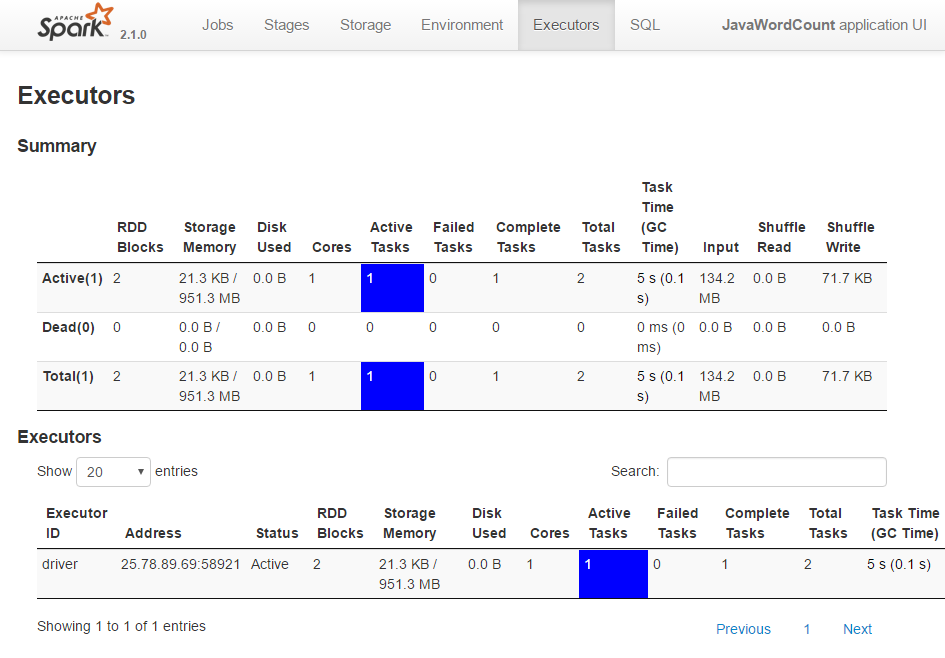
\includegraphics[width=\textwidth]{./bilder/spark_ui_worker.PNG}}
  \caption{Spark Web UI: Zusammenfassung der Worker}\label{fig:spark_ui_worker}
\end{figure}

%eventuell in die Performance section
\noindent
Speziell beim Thema SQL-Abfragen ist es enorm wichtig, dass man sich für die richtigen Anweisungen entscheidet, um langsame Operationen zu vermeiden. 
Wenige Änderungen an SQL-Abfragen können sehr große Geschwindigkeitsunterschiede bewirken.



\subsection{Besonderheiten bei der Speichernutzung}
Die Wahl einer geeigneten bzw. speicherplatzeffizienten Datenstruktur wird oftmals unterschätzt. Gerade bei großen Datenmengen und oftmals komprimierten Daten können schnell große Speichermengen benötigt werden. Das wird im folgenden Beispiel verdeutlicht.\\
Spark geht davon aus, dass eine Datei in Blöcke einer bestimmten Größe geladen wird. In der Regel beträgt die Blockgröße 128MB. Zu beachten ist jedoch, dass beim Dekomprimieren größere Blöcke entstehen können. So können aus 128MB schnell 3-4GB große Blöcke in dekomprimiertem Zustand werden. \\ 

\noindent
Um das Speichermanagement zu verbessern, wurde ein per-node allocator implementiert. Dieser verwaltet den Speicher auf einer Node. 
Der Speicher wird in drei Bereiche geteilt:
\begin{itemize}
	\item Speicher zum Verarbeiten der Daten
	\item Speicher für die hash-tables bei Joins oder Aggregations
	\item Speicher für \glqq{}unrolling\grqq{} Blöcke, um zu prüfen ob die einzulesenden Blöcke nach dem Entpacken immer noch klein genug sind, damit diese gecached werden können.
\end{itemize}
\noindent
Damit läuft das System robust für Anwendungsbereiche mit sehr vielen Maschinen sowie mit ganz wenigen \cite{ADD+15}.

\subsection{Netzwerk und I/O-Traffic}

%%schon Operationen bei denen über 8.000 Nodes involviert waren und über 1PB an Daten verarbeitet wurden durchgeführt.
Mit Apache Spark wurden Operationen, bei denen über 8.000 Nodes involviert waren und über 1PB an Daten verarbeitet wurden, durchgeführt. Das beansprucht die I/O Schicht enorm.
Um I/O Probleme zu vermeiden, bzw. diese besser zu beherrschen, wurde als Basis das Netty-Framework verwendet.
\begin{itemize}
	\item Zero-copy I/O:\\
	Daten werden direkt von der Festplatte zu dem Socket kopiert. Das vermeidet Last an der CPU bei Kontextwechseln und entlastet zusätzlich den JVM garbage collector\footnote{\textbf{garbage collector} kommt in Java zur automatischen Speicherbereinigung zum Einsatz}.
	\item Off-heap network buffer management:\\
	Netty verwaltet einige Speichertabellen außerhalb des Java Heap Speichers, um Probleme mit dem JVM garbage collector zu vermeiden.
	\item Mehrfache Verbindungen:\\
	Jeder Spark worker kann mehrere Verbindungen parallel bearbeiten.
\end{itemize}


\newpage
\section{Nutzung \& Verbreitung}
%%als wenn es nur eine einzige exotische Programmiersprache zur Nutzung gäbe. \\
Durch die Unterstützung der drei Programmiersprachen Scala, Python und Java ist die Arbeit mit Apache Spark einfacher, als wenn nur eine einzige exotische Programmiersprache verwendet werden könnte. \\



\noindent
Apache Spark unterstützt zudem noch verschiedene Datenquellen und Dateiformate.  Zu den Datenquellen zählen das Dateisystem S3\footnote{\textbf{S3} (Simple Storage Service) ist ein Filehosting-Dienst von Amazon der beliebig große Datenmengen speichern kann} von Amazon und das HDFS\footnote{\textbf{HDFS} (Hadoop Distributed File System) ist ein hochverfügbares Dateisystem zur Speicherung sehr großer Datenmengen}.
Die Dateiformate können strukturiert (z.B.: CSV, Object Files), semi-strukturiert (z.B.: JSON) und unstrukturiert (z.B.: Textdatei) sein.\\

\noindent
Zu den Mitwirkenden(Contributors) zählen über 400 Entwickler aus über 100 Unternehmen (Stand 2014). Es gibt über 500 produktive Installationen \cite{ADD+15}. \\ %PAPER: Scaling Spark in the Real World\\

\noindent
%http://spark.apache.org/community.html jährlich unter dem Namen Spark Summit Konferenzen statt. 
Seit einigen Jahren finden weltweit jährlich, unter dem Namen \glqq{}Spark Summit\grqq{} Konferenzen statt \cite{SPCOM}. \\


%"In einer Umfrage von Heise.de aus dem Jahr 2015 wurden 2.136 Teilnehmer zur Nutzung von Apache Spark befragt. 31 % der Befragten ..." (Eine Umfrage beauftragen? Tausenderpunkt; %2x Prozent bei der 31?^^)

%DONE: https://www.heise.de/developer/meldung/Big-Data-Umfrage-zur-Verbreitung-zu-Apache-Spark-2529126.html
\noindent
In einer Umfrage von Heise.de aus dem Jahr 2015 wurden 2.136 Teilnehmer zur Nutzung von Apache Spark befragt \cite{HEISEBIGDATA}. 31\% der Befragten gaben an, den Einsatz derzeit zu prüfen, 13\% nutzen bereits Apache Spark und 20\% planten den Einsatz noch in dem damaligen Jahr. Die Nutzung innerhalb verschiedener Berufsgruppen war sehr ähnlich. Mit 16\%  lag bei den Telekommunikationsunternehmen der Einsatz am höchsten.\\

\noindent
Bei denen, die es bereits im Einsatz haben, lag Scala bei den Programmiersprachen mit großem Abstand vorn. Eine detaillierte Übersicht ist in \autoref{fig:nutzung} zu sehen.
\begin{figure}[h]
  \centering
  \fbox{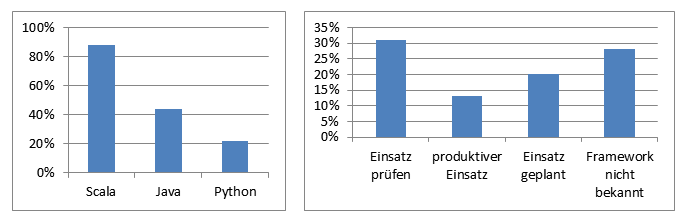
\includegraphics[width=140mm]{./excel/Nutzung.png}}
  \caption{Verbreitung \& Einsatz}\label{fig:nutzung}
\end{figure}
 
\newpage
\chapter{Fazit} 
\large
Lorem ipsum dolor sit amet, consetetur sadipscing elitr, sed diam nonumy eirmod tempor invidunt ut labore et dolore magna aliquyam erat, sed diam voluptua. At vero eos et accusam et justo duo dolores et ea rebum. Stet clita kasd gubergren, no sea takimata sanctus est Lorem ipsum dolor sit amet. Lorem ipsum dolor sit amet, consetetur sadipscing elitr, sed diam nonumy eirmod tempor invidunt ut labore et dolore magna aliquyam erat, sed diam voluptua. At vero eos et accusam et justo duo dolores et ea rebum. Stet clita kasd gubergren, no sea takimata sanctus est Lorem ipsum dolor sit amet. Lorem ipsum dolor sit amet, consetetur sadipscing elitr, sed diam nonumy eirmod tempor invidunt ut labore et dolore magna aliquyam erat, sed diam voluptua. At vero\footnote{At vero: ist eine Kleine Fußnaote} eos et accusam et justo duo dolores et ea rebum. Stet clita kasd gubergren, no sea takimata sanctus est Lorem ipsum dolor sit amet.   



Duis autem vel eum iriure dolor in hendrerit in vulputate velit esse molestie consequat, vel illum dolore eu feugiat nulla facilisis at vero eros et accumsan et iusto odio dignissim qui blandit praesent luptatum zzril delenit augue duis dolore te feugait nulla facilisi. Lorem ipsum dolor sit amet, consectetuer adipiscing elit, sed diam nonummy nibh euismod tincidunt ut laoreet dolore magna aliquam erat volutpat.   

Ut wisi enim ad minim veniam, quis nostrud exerci tation ullamcorper suscipit lobortis nisl ut aliquip ex ea commodo consequat. Duis autem vel eum iriure dolor in hendrerit in vulputate velit esse molestie consequat, vel illum dolore eu feugiat nulla facilisis at vero eros et accumsan et iusto odio dignissim qui blandit praesent luptatum zzril delenit augue duis dolore te feugait nulla facilisi.   

Nam liber tempor cum soluta nobis eleifend option congue nihil imperdiet doming id quod mazim placerat facer possim assum. Lorem ipsum dolor sit amet, consectetuer adipiscing elit, sed diam nonummy nibh euismod tincidunt ut laoreet dolore magna aliquam erat volutpat. Ut wisi enim ad minim veniam, quis nostrud exerci tation ullamcorper suscipit lobortis nisl ut aliquip ex ea commodo consequat.   

Duis autem vel eum iriure dolor in hendrerit in vulputate velit esse molestie consequat, vel illum dolore eu feugiat nulla facilisis.   

At vero eos et accusam et justo duo dolores et ea rebum. Stet clita kasd gubergren, no sea takimata sanctus est Lorem ipsum dolor sit amet. Lorem ipsum dolor sit amet, consetetur sadipscing elitr, sed diam nonumy eirmod tempor invidunt ut labore et dolore magna aliquyam erat, sed diam voluptua. At vero eos et accusam et justo duo dolores et ea rebum. Stet clita kasd gubergren, no sea takimata sanctus est Lorem ipsum dolor sit amet. Lorem ipsum dolor sit amet, consetetur sadipscing elitr, At accusam aliquyam diam diam dolore dolores duo eirmod eos erat, et nonumy sed tempor et et invidunt justo labore Stet clita ea et gubergren, kasd magna no rebum. sanctus sea sed takimata ut vero voluptua. est Lorem ipsum dolor sit amet. Lorem ipsum dolor sit amet, consetetur

Lorem ipsum dolor sit amet, consetetur sadipscing elitr, sed diam nonumy eirmod tempor invidunt ut labore et dolore magna aliquyam erat, sed diam voluptua. At vero eos et accusam et justo duo dolores et ea rebum. Stet clita kasd gubergren, no sea takimata sanctus est Lorem ipsum dolor sit amet. Lorem ipsum dolor sit amet, consetetur sadipscing elitr, sed diam nonumy eirmod tempor invidunt ut labore et dolore magna aliquyam erat, sed diam voluptua. At vero eos et accusam et justo duo dolores et ea rebum. Stet clita kasd gubergren, no sea takimata sanctus est Lorem ipsum dolor sit amet. Lorem ipsum dolor sit amet, consetetur sadipscing elitr, sed diam nonumy eirmod tempor invidunt ut labore et dolore magna aliquyam erat, sed diam voluptua. At vero eos et accusam et justo duo dolores et ea rebum. Stet clita kasd gubergren, no sea takimata sanctus est Lorem ipsum dolor sit amet.   

Duis autem vel eum iriure dolor in hendrerit in vulputate velit esse molestie consequat, vel illum dolore eu feugiat nulla facilisis at vero eros et accumsan et iusto odio dignissim qui blandit praesent luptatum zzril delenit augue duis dolore te feugait nulla facilisi. Lorem ipsum dolor sit amet, consectetuer adipiscing elit, sed diam nonummy nibh euismod tincidunt ut laoreet dolore magna aliquam erat volutpat.   

Ut wisi enim ad minim veniam, quis nostrud exerci tation ullamcorper suscipit lobortis nisl ut aliquip ex ea commodo consequat. Duis autem vel eum iriure dolor in hendrerit in vulputate velit esse molestie consequat, vel illum dolore eu feugiat nulla facilisis at vero eros et accumsan et iusto odio dignissim qui blandit praesent luptatum zzril delenit augue duis dolore te feugait nulla facilisi.   

Nam liber tempor cum soluta nobis eleifend option congue nihil imperdiet doming id quod mazim placerat facer possim assum. Lorem ipsum dolor sit amet, consectetuer adipiscing elit, sed diam nonummy nibh euismod tincidunt ut laoreet dolore magna aliquam erat volutpat. Ut wisi enim ad minim veniam, quis nostrud exerci tation ullamcorper suscipit lobortis nisl ut aliquip ex ea commodo consequat.   

Duis autem vel eum iriure dolor in hendrerit in vulputate velit esse molestie consequat, vel illum dolore eu feugiat nulla facilisis.   

At vero eos et accusam et justo duo dolores et ea rebum. Stet clita kasd gubergren, no sea takimata sanctus est Lorem ipsum dolor sit amet. Lorem ipsum dolor sit amet, consetetur sadipscing elitr, sed diam nonumy eirmod tempor invidunt ut labore et dolore magna aliquyam erat, sed diam voluptua. At vero eos et accusam et justo duo dolores et ea rebum. Stet clita kasd gubergren, no sea takimata sanctus est Lorem ipsum dolor sit amet. Lorem ipsum dolor sit amet, consetetur sadipscing elitr, At accusam aliquyam diam diam dolore dolores duo eirmod eos erat, et nonumy sed tempor et et invidunt justo labore Stet clita ea et gubergren, kasd magna no rebum. sanctus sea sed takimata ut vero voluptua. est Lorem ipsum dolor sit amet. Lorem ipsum dolor sit amet, consetetur

Lorem ipsum dolor sit amet, consetetur sadipscing elitr, sed diam nonumy eirmod tempor invidunt ut labore et dolore magna aliquyam erat, sed diam voluptua. At vero eos et accusam et justo duo dolores et ea rebum. Stet clita kasd gubergren, no sea takimata sanctus est Lorem ipsum dolor sit amet. Lorem ipsum dolor sit amet, consetetur sadipscing elitr, sed diam nonumy eirmod tempor invidunt ut labore et dolore magna aliquyam erat, sed diam voluptua. At vero eos et accusam et justo duo dolores et ea rebum. Stet clita kasd gubergren, no sea takimata sanctus est Lorem ipsum dolor sit amet. Lorem ipsum dolor sit amet, consetetur sadipscing elitr, sed diam nonumy eirmod tempor invidunt ut labore et dolore magna aliquyam erat, sed diam voluptua. At vero eos et accusam et justo duo dolores et ea rebum. Stet clita kasd gubergren, no sea takimata sanctus est Lorem ipsum dolor sit amet.   

Duis autem vel eum iriure dolor in hendrerit in vulputate velit esse molestie consequat, vel illum dolore eu feugiat nulla facilisis at vero eros et accumsan et iusto odio dignissim qui blandit praesent luptatum zzril delenit augue duis dolore te feugait nulla facilisi. Lorem ipsum dolor sit amet, consectetuer adipiscing elit, sed diam nonummy nibh euismod tincidunt ut laoreet dolore magna aliquam erat volutpat.   

Ut wisi enim ad minim veniam, quis nostrud exerci tation ullamcorper suscipit lobortis nisl ut aliquip ex ea commodo consequat. Duis autem vel eum iriure dolor in hendrerit in vulputate velit esse molestie consequat, vel illum dolore eu feugiat nulla facilisis at vero eros et accumsan et iusto odio dignissim qui blandit praesent luptatum zzril delenit augue duis dolore te feugait nulla facilisi.   

Nam liber tempor cum soluta nobis eleifend option congue nihil imperdiet doming id quod mazim placerat facer possim assum. Lorem ipsum dolor sit amet, consectetuer adipiscing elit, sed diam nonummy nibh euismod tincidunt ut laoreet dolore magna aliquam erat volutpat. Ut wisi enim ad minim veniam, quis nostrud exerci tation ullamcorper suscipit lobortis nisl ut aliquip ex ea commodo consequat.   

Duis autem vel eum iriure dolor in hendrerit in vulputate velit esse molestie consequat, vel illum dolore eu feugiat nulla facilisis.   

At vero eos et accusam et justo duo dolores et ea rebum. Stet clita kasd gubergren, no sea takimata sanctus est Lorem ipsum dolor sit amet. Lorem ipsum dolor sit amet, consetetur sadipscing elitr, sed diam nonumy eirmod tempor invidunt ut labore et dolore magna aliquyam erat, sed diam voluptua. At vero eos et accusam et justo duo dolores et ea rebum. Stet clita kasd gubergren, no sea takimata sanctus est Lorem ipsum dolor sit amet. Lorem ipsum dolor sit amet, consetetur sadipscing elitr, At accusam aliquyam diam diam dolore dolores duo eirmod eos erat, et nonumy sed tempor et et invidunt justo labore Stet clita ea et gubergren, kasd magna no rebum. sanctus sea sed takimata ut vero voluptua. est Lorem ipsum dolor sit amet. Lorem ipsum dolor sit amet, consetetur

Lorem ipsum dolor sit amet, consetetur sadipscing elitr, sed diam nonumy eirmod tempor invidunt ut labore et dolore magna aliquyam erat, sed diam voluptua. At vero eos et accusam et justo duo dolores et ea rebum. Stet clita kasd gubergren, no sea takimata sanctus est Lorem ipsum dolor sit amet. Lorem ipsum dolor sit amet, consetetur sadipscing elitr, sed diam nonumy eirmod tempor invidunt ut labore et dolore magna aliquyam erat, sed diam voluptua. At vero eos et accusam et justo duo dolores et ea rebum. Stet clita kasd gubergren, no sea takimata sanctus est Lorem ipsum dolor sit amet. Lorem ipsum dolor sit amet, consetetur sadipscing elitr, sed diam nonumy eirmod tempor invidunt ut labore et dolore magna aliquyam erat, sed diam voluptua. At vero eos et accusam et justo duo dolores et ea rebum. Stet clita kasd gubergren, no sea takimata sanctus est Lorem ipsum dolor sit amet.   

Duis autem vel eum iriure dolor in hendrerit in vulputate velit esse molestie consequat, vel illum dolore eu feugiat nulla facilisis at vero eros et accumsan et iusto odio dignissim qui blandit praesent luptatum zzril delenit augue duis dolore te feugait nulla facilisi. Lorem ipsum dolor sit amet, consectetuer adipiscing elit, sed diam nonummy nibh euismod tincidunt ut laoreet dolore magna aliquam erat volutpat.   

Ut wisi enim ad minim veniam, quis nostrud exerci tation ullamcorper suscipit lobortis nisl ut aliquip ex ea commodo consequat. Duis autem vel eum iriure dolor in hendrerit in vulputate velit esse molestie consequat, vel illum dolore eu feugiat nulla facilisis at vero eros et accumsan et iusto odio dignissim qui blandit praesent luptatum zzril delenit augue duis dolore te feugait nulla facilisi.   

Nam liber tempor cum soluta nobis eleifend option congue nihil imperdiet doming id quod mazim placerat facer possim assum. Lorem ipsum dolor sit amet, consectetuer adipiscing elit, sed diam nonummy nibh euismod tincidunt ut laoreet dolore magna aliquam erat volutpat. Ut wisi enim ad minim veniam, quis nostrud exerci tation ullamcorper suscipit lobortis nisl ut aliquip ex ea commodo consequat.   

Duis autem vel eum iriure dolor in hendrerit in vulputate velit esse molestie consequat, vel illum dolore eu feugiat nulla facilisis.   

At vero eos et accusam et justo duo dolores et ea rebum. Stet clita kasd gubergren, no sea takimata sanctus est Lorem ipsum dolor sit amet. Lorem ipsum dolor sit amet, consetetur sadipscing elitr, sed diam nonumy eirmod tempor invidunt ut labore et dolore magna aliquyam erat, sed diam voluptua. At vero eos et accusam et justo duo dolores et ea rebum. Stet clita kasd gubergren, no sea takimata sanctus est Lorem ipsum dolor sit amet. Lorem ipsum dolor sit amet, consetetur sadipscing elitr, At accusam aliquyam diam diam dolore dolores duo eirmod eos erat, et nonumy sed tempor et et invidunt justo labore Stet clita ea et gubergren, kasd magna no rebum. sanctus sea sed takimata ut vero voluptua. est Lorem ipsum dolor sit amet. Lorem ipsum dolor sit amet, consetetur

Lorem ipsum dolor sit amet, consetetur sadipscing elitr, sed diam nonumy eirmod tempor invidunt ut labore et dolore magna aliquyam erat, sed diam voluptua. At vero eos et accusam et justo duo dolores et ea rebum. Stet clita kasd gubergren, no sea takimata sanctus est Lorem ipsum dolor sit amet. Lorem ipsum dolor sit amet, consetetur sadipscing elitr, sed diam nonumy eirmod tempor invidunt ut labore et dolore magna aliquyam erat, sed diam voluptua. At vero eos et accusam et justo duo dolores et ea rebum. Stet clita kasd gubergren, no sea takimata sanctus est Lorem ipsum dolor sit amet. Lorem ipsum dolor sit amet, consetetur sadipscing elitr, sed diam nonumy eirmod tempor invidunt ut labore et dolore magna aliquyam erat, sed diam voluptua. At vero eos et accusam et justo duo dolores et ea rebum. Stet clita kasd gubergren, no sea takimata sanctus est Lorem ipsum dolor sit amet.   

Duis autem vel eum iriure dolor in hendrerit in vulputate velit esse molestie consequat, vel illum dolore eu feugiat nulla facilisis at vero eros et accumsan et iusto odio dignissim qui blandit praesent luptatum zzril delenit augue duis dolore te feugait nulla facilisi. Lorem ipsum dolor sit amet, consectetuer adipiscing elit, sed diam nonummy nibh euismod tincidunt ut laoreet dolore magna aliquam erat volutpat.   

Ut wisi enim ad minim veniam, quis nostrud exerci tation ullamcorper suscipit lobortis nisl ut aliquip ex ea commodo consequat. Duis autem vel eum iriure dolor in hendrerit in vulputate velit esse molestie consequat, vel illum dolore eu feugiat nulla facilisis at vero eros et accumsan et iusto odio dignissim qui blandit praesent luptatum zzril delenit augue duis dolore te feugait nulla facilisi.   

Nam liber tempor cum soluta nobis eleifend option congue nihil imperdiet doming id quod mazim placerat facer possim assum. Lorem ipsum dolor sit amet, consectetuer adipiscing elit, sed diam nonummy nibh euismod tincidunt ut laoreet dolore magna aliquam erat volutpat. Ut wisi enim ad minim veniam, quis nostrud exerci tation ullamcorper suscipit lobortis nisl ut aliquip ex ea commodo consequat.   

Duis autem vel eum iriure dolor in hendrerit in vulputate velit esse molestie consequat, vel illum dolore eu feugiat nulla facilisis.   

At vero eos et accusam et justo duo dolores et ea rebum. Stet clita kasd gubergren, no sea takimata sanctus est Lorem ipsum dolor sit amet. Lorem ipsum dolor sit amet, consetetur sadipscing elitr, sed diam nonumy eirmod tempor invidunt ut labore et dolore magna aliquyam erat, sed diam voluptua. At vero eos et accusam et justo duo dolores et ea rebum. Stet clita kasd gubergren, no sea takimata sanctus est Lorem ipsum dolor sit amet. Lorem ipsum dolor sit amet, consetetur sadipscing elitr, At accusam aliquyam diam diam dolore dolores duo eirmod eos erat, et nonumy sed tempor et et invidunt justo labore Stet clita ea et gubergren, kasd magna no rebum. sanctus sea sed takimata ut vero voluptua. est Lorem ipsum dolor sit amet. Lorem ipsum dolor sit amet, consetetur 
\newpage
\chapter{Ausblick \& Weiterentwicklung}  
\newpage
\chapter{Anhang}  
\newpage
\chapter{Literaturverzeichnis}  



\end{document}

